\chapter{Development}
\label{chap:dev}

This chapter discusses the tools and methodologies employed in the code development of this system. 

\section{Development  Language}

The framework was written in Python 3.6, which at the time of submission is the latest supported Python release. It is worth noting that the research implementation of the user simulator described in \cite{li_usersim} was written in Python 2. Python 3 is the preferred version for production Python products. Most major data science and machine learning research Python libraries no longer support Python 2. Python 3 provides many useful features and performance upgrades that make writing and deploying python projects more efficient and effective. In addition to updated syntax that allows for more expressive coding, the standard library was extended to support new data types (ordered dictionaries, enumerated types, data classes). Additionally, Python 3.5 introduced type annotation, which allows for the writing of cleaner, better documented, and unambiguous code. 

Socrates Sim was written to adhere to the PEP8 standard and all method signatures have type annotations. The hope is that good software documentation and standard coding styles will allow future contributors to easily debug, modify, and build new modules for the framework. 

\section{Development  Tools}

Socrates Sim was developed using the PyCharm IDE. Pycharm was selected for its ease of use, Python debugging tools, and integration with Github. Various Python libraries were used in the development of the framework. The following third-party Python packages have a significant impact on the development of the framework:

\begin{itemize}
	\item yaml: The yaml library provides a set of functions to read and write yaml files. It was primarily for the loading and saving of the various configuration files. 
	\item json: The json library provides a set of functions to read and write json files. It was primarily used for the loading and saving of various configuration files and the serialization of the simulated dialogs. 
	\item spacy and nltk: Spacy and NLTK are natural language processing libraries that provide standard NLP tools like part of speech tagging, dependency parsing and, named entity recognition. They were used primarily for developing the base natural language understanding and natural language generation models. 
	\item pandas: The pandas library provides robust, efficient, and flexible data structures that can be used for data science. The pandas dataframe was used to represent the knowledge base in-memory and execute various logical queries.
	\item OpenNMT: OpenNMT is Python library used for neural machine translation. OpenNMT was used to train the nlu and nlg models.
	\item memory-profiler: This library was used to measure the memory consumption of the framework.  
\end{itemize}

The code base is stored on Github.com and uses git for version control and bug tracking. Github is an online cloud-based software platform used for sharing and hosting code bases. Github provides various collaboration and version tracking features.

\chapter{Results}

This chapter discusses the performance tests and results of the Socrates Simulator.

\section{Experiment Overview and Setup}

 Socrates Simulator is novel as an open source end-to-end dialog simulation framework. As a result, it was challenging to develop a meaningful benchmark for evaluation. We ultimately chose the TC-Bot framework, which is the research implementation of end-to-end neural dialog framework described in \cite{li_end_to_end}. We measured two aspects of the Socrates simulator, its scalability and its memory consumption over the course of running multiple simulations. The goal was to show that Socrates Sim is generally usable and that overall performance does not significantly degrade with expanded usage across different domains and increased simulation runs. 
 
 TC-Bot is the academic inspiration for this project. TC-Bot shares similar objectives for the training and evaluation of task-completion dialog agents. However, there are several key distinctions between TC-Bot and Socrates Sim. First, the neural architecture for training the dialog agent is tightly coupled with the overall framework for TC-Bot. Second, TC-Bot was hardcoded for a limited movie booking use case. Finally, the training data used by TC-Bot was collected with Amazon Turk and not publicly released. They did provide some of the intermediate representations (Python 2.7 encoded pickle files) of the data (e.g., dialog acts, slot values, etc). However, these intermediate representations were optimized for their specific use case and were unusable for general usage. Adapting TC-Bot to a new domain would have required non-trivial work rewriting the neural framework, which is outside of the scope of this project. To test TC-Bot, we ran the framework as is, with no changes to the domain or underlying framework. 

Initially, performance testing was conducted on a MacBook Pro laptop with a core i7 processor and 16 GB of memory. However, TC-Bot's performance was significantly reduced due to its neural-architecture, which performed best on a gpu (graphical processing unit) enabled machine. In order to ensure a fair comparison, all performance tests were run on a gpu enabled server. Specifically, the server was running Ubuntu 14.04, with a core i9 3.3 ghz 10 core cpu and  64 gb of RAM. Additionally, the server had two gpus, a Titan Pascal and a Titan XP 12 gb GPU. 

A master script was written to coordinate iteratively calling each framework with a variable simulation count parameter. Each time, the framework is be called as an isolated subprocess of the master script to ensure more accurate measurements. 

\section{Runtime Performance Experiment and Results}

The goal of these tests was to measure how effectively the framework's runtime scaled with increased simulation rounds. Runtime is defined here as the elapsed time taken to run \textit{n} simulations, where \textit{n} is a positive integer. Starting with one simulation, we iteratively increased the simulations by 500, until we ran a total of 50,000 simulated dialogs. We do not capture the write time to save the simulated dialogs to disk. This is usually a linear cost proportional to the size of the stored dialogs in memory. 

In total, we ran six different performances tests. Four tests were run on the Socrates Sim framework and two on the TC-Bot framework. 
\begin{figure}[h!]
	\centering
	\label{fig:rules_test}
	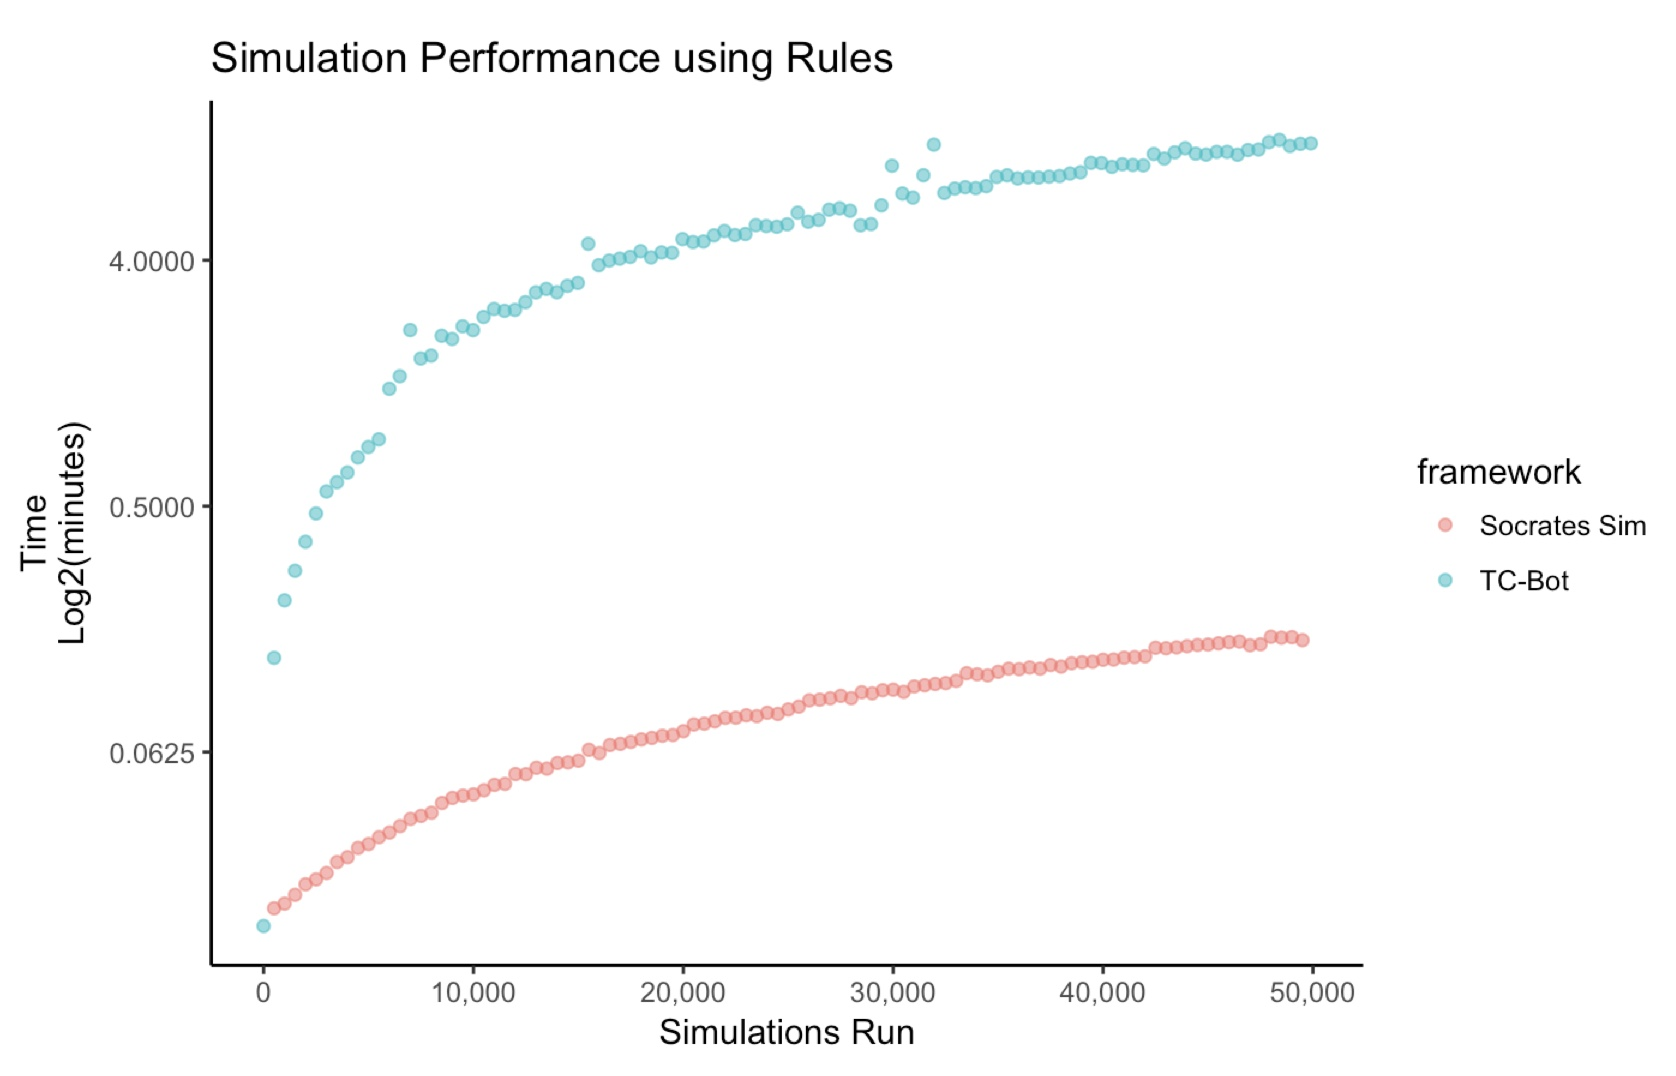
\includegraphics[width=\linewidth]{diagrams/rules_perf_test.jpeg}
	\caption{ Runtime of Socrates Sim vs TC-Bot with rule based user simulator.}
\end{figure}

For the first two tests, we compare the performance of end-to-end dialog simulations using a rules-based approach. For both frameworks, we use the movie booking use case. In the Socrates Simulator, both the dialog agent and user simulator are rules-based speakers and have rules-based nlu and nlg modules. In TC-Bot, the user simulator is rules-based and the dialog agent is a DQNN neural model that is being trained on a reward signal after each simulation round.  Both frameworks have a \textit{O(N)} runtime as the simulation sizes grew, as shown in Figure \ref{fig:rules_test}. However, Socrates Sim performed overall more efficiently, taking on average about 1 minute and 51 seconds to run 50,000 simulations. In contrast, TC-Bot took on average 10 minutes and 44 seconds. A large part of this can be attributed to the fact that TC-Bot tightly couples training the dialog agent with the dialog simulation. That is, after each round, TC-Bot runs stochastic gradient descent on the reward function in order to inform the dialog agent's action in the proceeding round. 

For the next two tests, we compare the performances of both frameworks using model-based actors. As with the first two experiments, we are evaluating in the movie booking use case. For Socrates Sim, we initially use the OpenNMT trained nlu and nlg module for the user simulator and dialog agent. Since OpenNMT does not support programmatic access, our initial performance tests were very poor. It took Socrates Sim about 50 minutes to run 1,000 simulations. Each call to OpenNMT required launching a new subprocess, invoking OpenNMT anew, and running the prediction. 

A preloaded model in memory would be more efficient. Therefore we switched to evaluating the performance of Socrates Sim using the \cite{brownlee_2017} neural machine translations models. The benefit of this model is that it can be invoked programmatically. At the very initial load, neural models (serialized as hd5 files) are loaded into memory. Each call to the model involved a small preprocessing cost and an additional cost to do a forward pass through the network.  On average, it took about 1 minute and 21 seconds to run 1,000 simulations. In contrast, we find that TC-Bot does perform much more efficiently. While its growth is still linear, it can run 1,000 simulations in about 30 seconds. For running neural models, TC-Bot is about 3 times faster. 

\begin{figure}[h!]
	\centering
	\label{fig:nm_test}
	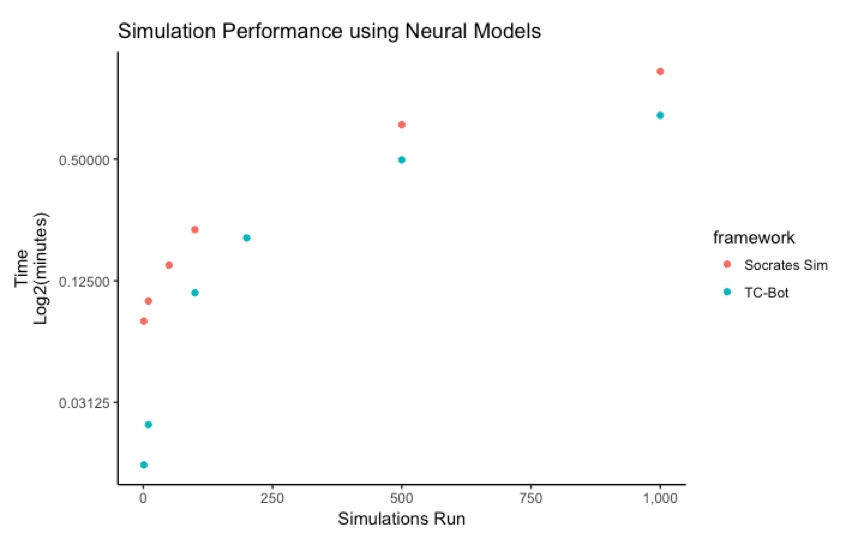
\includegraphics[width=\linewidth]{diagrams/neural_perf_test.jpeg}
	\caption{ Runtime of Socrates Sim vs TC-Bot with model-based user simulator.}
\end{figure}

 Finally, our last set of experiments involve testing runtime performance across domains. As TC-Bot is hard-coded for the movie booking use case, it was not included in our performance tests. In Figure \ref{fig:perf_cd_test}, we see that there is variation between domains. Both have linear growth, though the movie domain performs more efficiently, taking about 30 seconds to generate 50,000 simulations. What we find is that the overall performance of the framework is tied to the complexity of the domain and speaker classes. From a general usability point of view, we assert that framework scales predictably and is usable. End-to-end, it takes about two minutes to run 50,000 simulations for the restaurant domain, which is reasonable. 
 
  \begin{figure}[h!]
 	\label{fig:perf_cd_test}
 	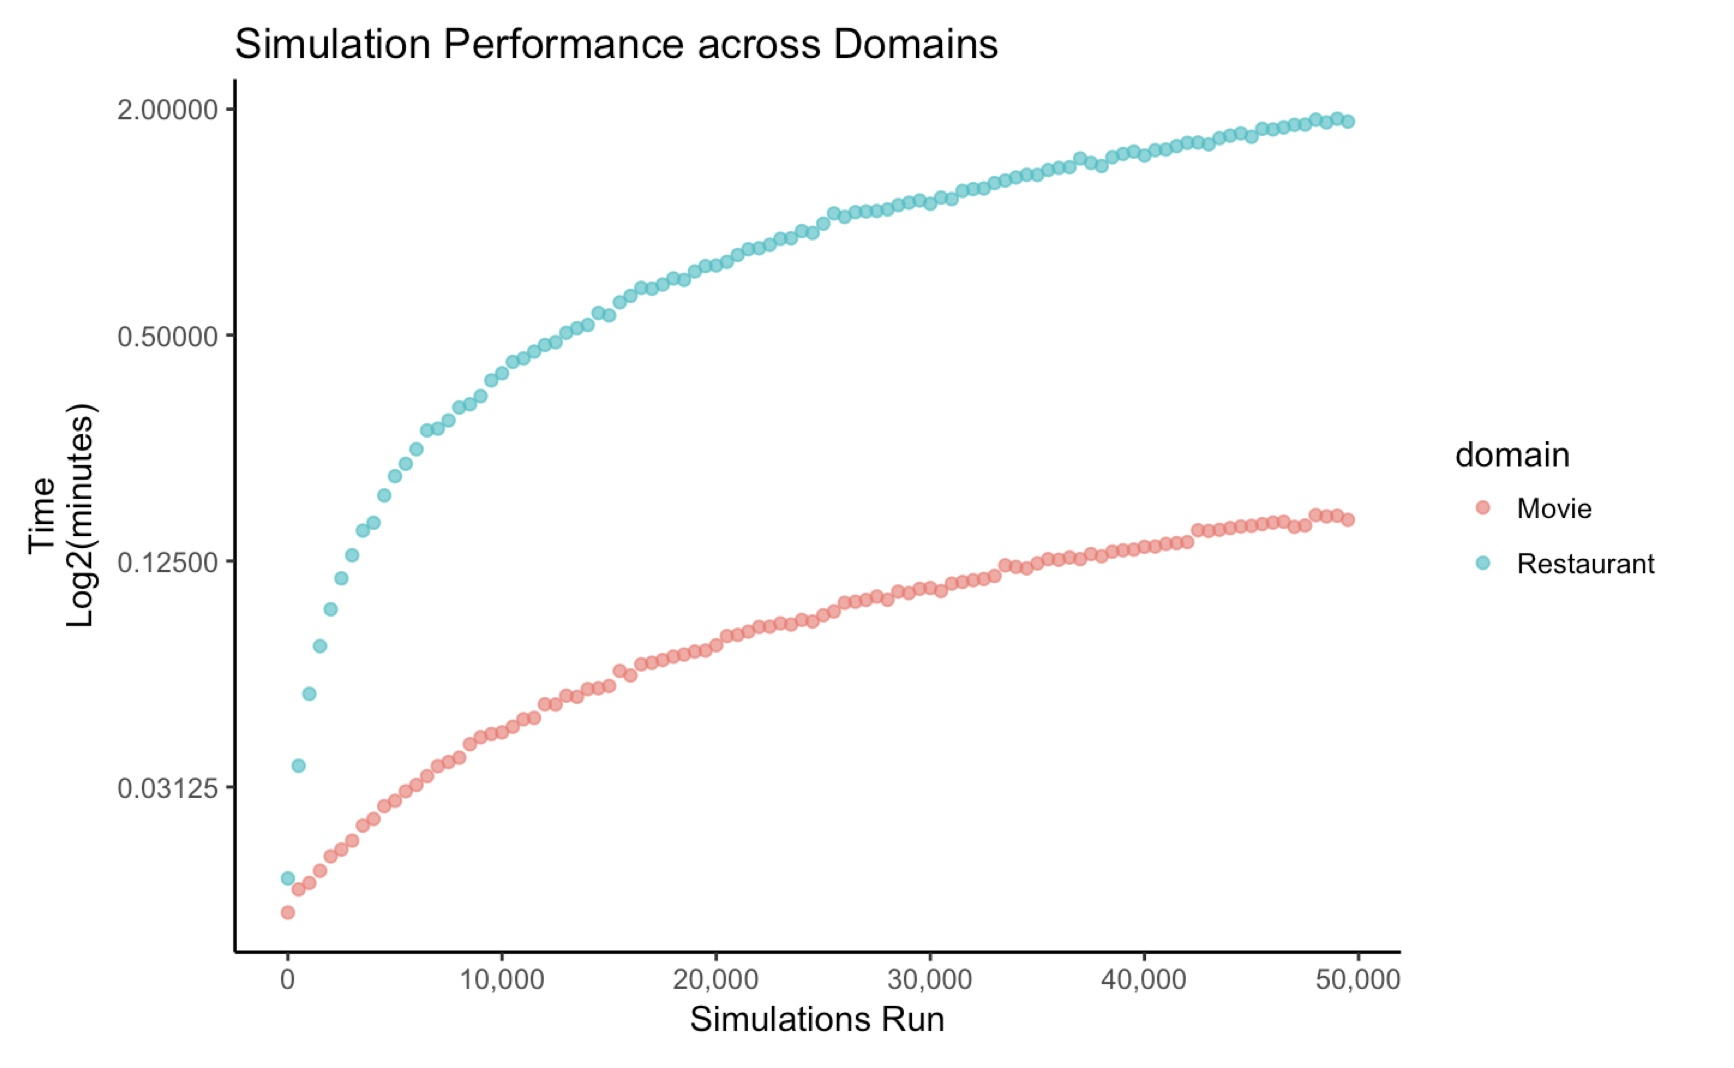
\includegraphics[width=\linewidth]{diagrams/domain_perf.jpeg}
 	\caption{ Runtime performance across domains.}
 \end{figure}

Growth is linear across all frameworks and domains. In the table below, we measure the average cost per simulation and rank all the framework/domain combinations from fastest to the slowest. The rules-based models for Socrates Sim significantly outperforms TC-Bot. In contrast, the model-based TC-Bot is about three times faster that Socrates Sim. Finally, rules-based approaches,in general, are more efficient to run. 

\begin{figure}[h!]
	\centering
	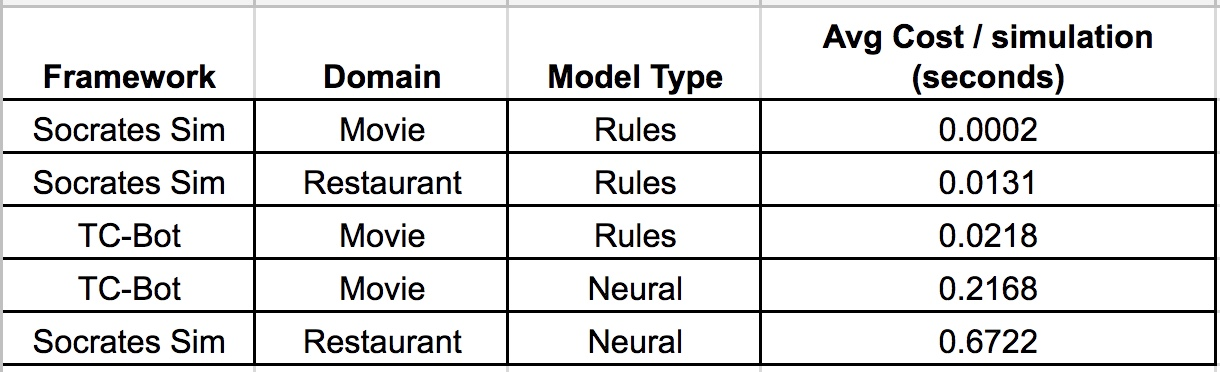
\includegraphics[width=\linewidth]{diagrams/avg_cost.jpeg}	
	\caption{ Average cost to run a single simulation.}
	\label{fig:avg_cost}
\end{figure}

 There is an opportunity to further improve overall performance. As the simulations can run independently, we can introduce multi-threading and leverage the multi-core cpus for parallel processing. The dialog manager can be extended to support a thread pool and spawn multiple threads to run simulations in parallel. This could significantly improve performance if the researcher needs to generate hundreds of thousands or millions of simulations.  

\section{Memory Consumption Experiment and Results}

The next set of tests involve measuring maximum memory consumption of the framework when generating multiple dialog simulations. The goal is to show that Socrates Simulator consumes memory reasonably and is usable. Like the performance tests above, we ran a total of 6 tests to evaluate memory consumption. Four tests were on the Socrates Sim framework and two on the TC-Bot framework.

To measure memory consumption, we used the Python based \textit{memory-profiler} tool. The tool is invoked via command lined and runs the program to be evaluated as an internal sub-process. Over the duration of the observed program's runtime, \textit{memory-profiler} uses the \textit{psustil} tool to probe the operating system for information about CPU usage, running processes, and resource utilization. \textit{Memory-profiler} will log memory usage at predefined increments until the program finishes running. 

\begin{figure}[h!]
	\label{fig:mem_usage_rules}
	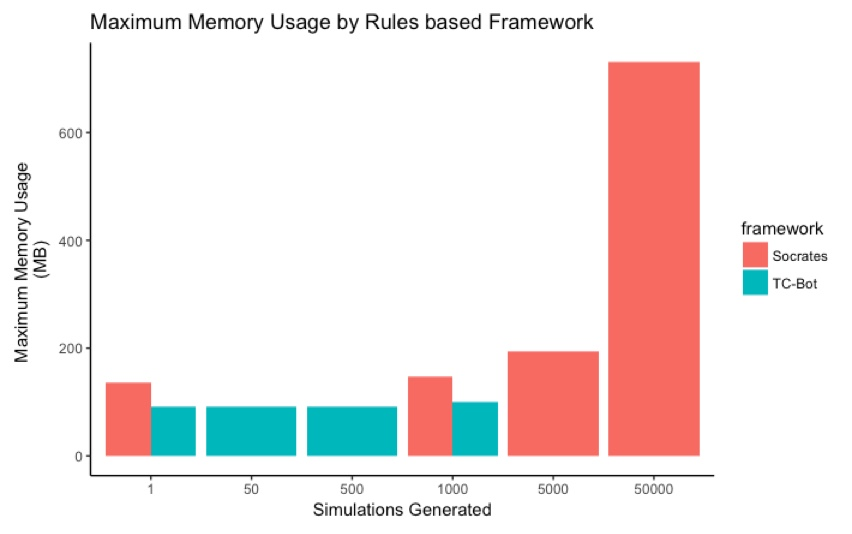
\includegraphics[width=\linewidth]{diagrams/mem_usage_rules.jpeg}
	\caption{ Memory usage of Socrates Sim vs TC-Bot with rule based user simulator.}
\end{figure}

For the first test, we looked at the maximum memory usage of both frameworks when using rule-based actors for the movie domain. Figure \ref{fig:mem_usage_rules} shows relative performance of both frameworks. TC-Bot performs significantly better, capping at about 150 MB of overall memory usage over the course all simulations run. Running up to 5,000 simulations, Socrates Sim uses under 200 MB of memory. At the 50,000 simulations, memory usage does significantly increase to about 700 MB. It is worth noting that this much memory is only utilized at the tail end of Socrates Sim's runtime. This likely due to the fact that the dialog manager has not serialized the generated dialogs and is holding them in memory until all simulations have run.  

\begin{figure}[h!]
		\centering
	\label{fig:mem_usage_nm}
	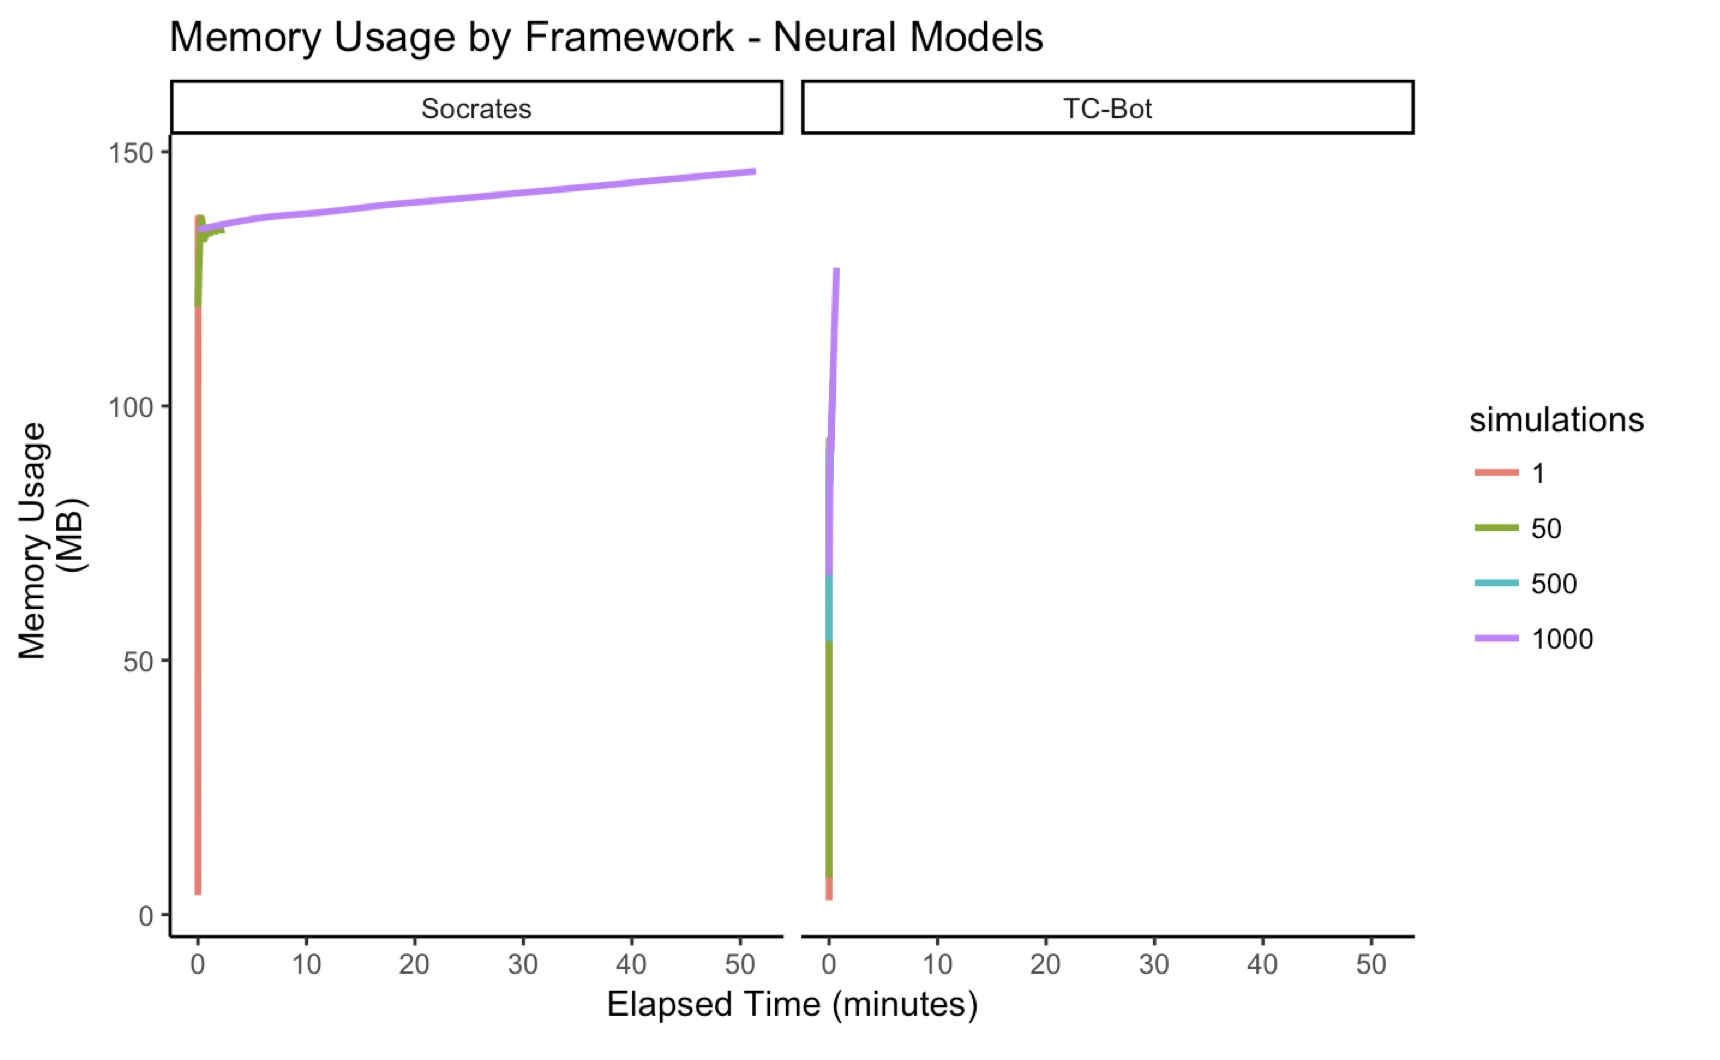
\includegraphics[width=\linewidth]{diagrams/mem_usage_neural.jpeg}
	\caption{ Memory usage of Socrates Sim vs TC-Bot with model-based user simulator. }
\end{figure}

In Figure \ref{fig:mem_usage_nm}, we see the results for memory consumption when using neural models. Note, that we used the restaurant domain for reasons explained above. Overall, both TC-Bot and Socrates Sim use a little under 150 MB. While runtime performance is drastically different, with TC-Bot running more efficiently overall, both frameworks have similar memory usage patterns. 

Finally, in Figure \ref{fig:mem_usage_cd}, we see the results for memory usage across the restaurant and movie domains for Socrates Sim. Under 10,000 simulations, we found total memory usage caps around 250 MB. 

\begin{figure}[h!]
		\centering
	\label{fig:mem_usage_cd}
	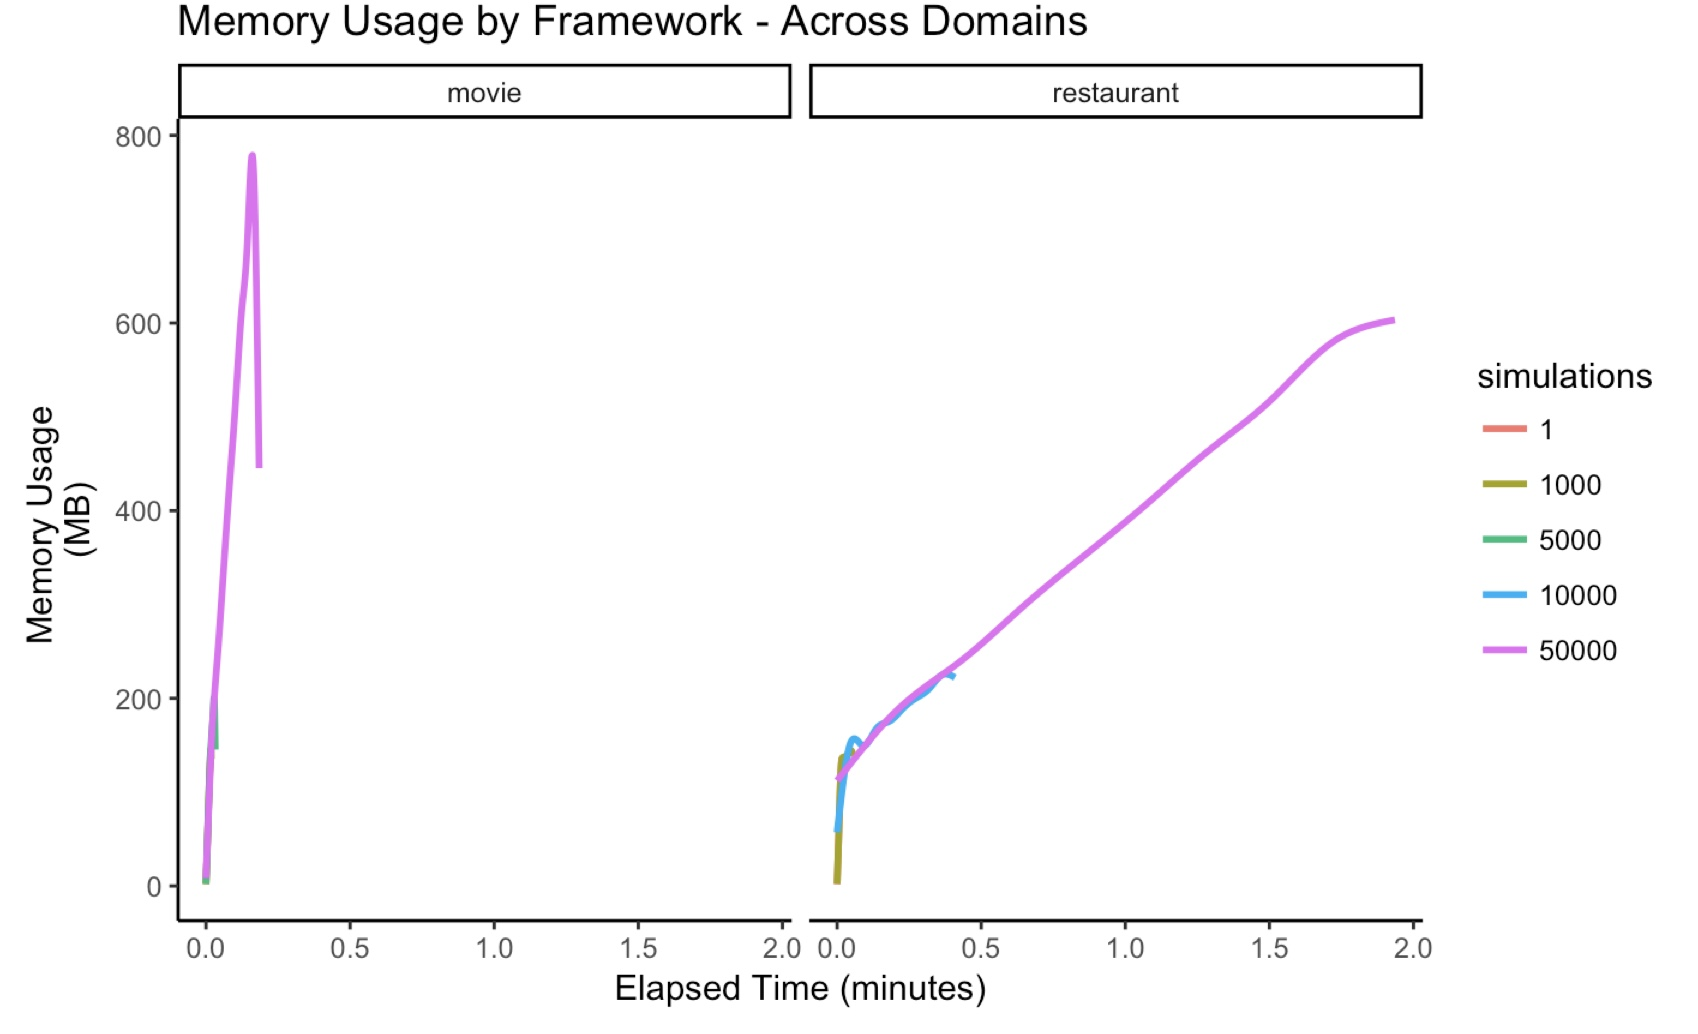
\includegraphics[width=\linewidth]{diagrams/mem_usage_domains.jpeg}
	\caption{ Memory usage across domains for Socrates Sim.}
\end{figure}

All the tests reveal a small oversight in the Socrates Simulator design. The tests show that memory usage grows linearly with the number of simulations run. This is due to the fact the dialog manager does not serialize the generated dialogs until all simulations are run. This is a minor design choice, which can be updated to have the dialog manager periodically serialize the queue of generated dialogs and reset the queue. 

Accounting for the serialization issue, the overall memory usage for Socrates Sim is reasonable. In small simulations (under 50,000), Socrates Sim has a similar memory usage profile to TC-Bot. We believe Socrates Simulator is usable and provides predictable performance and memory utilization. For rules-based use case, Socrates Sim is quite efficient. Accounting for the complexity of the rules, the researcher is able to run thousands of simulations in a matter of minutes. Overall, both the performance tests and memory utilization tests show that Socrates Simulator can be used for most reasonable use cases. 
%%% Local Variables: 
%%% mode: latex
%%% TeX-master: "main"
%%% End: 
